\documentclass[12pt]{article}

\usepackage{amsmath, amssymb}
\usepackage[margin=1in]{geometry}
\usepackage{helvet}
\renewcommand{\familydefault}{\sfdefault}
\def\newrule#1#2#3{\begin{center}
    {#1} \\
    \line(1,0){300} {}{}{}{}{}{}{} [{#3}]\\
    {#2}
\end{center}}

\begin{document}
\def\assignment{Homework 04}

\pagenumbering{gobble}
\noindent{\large COSC 4200 \hfill Name: \underline{Jacob Tuttle} \\ Computability and Complexity}
\begin{center}
    {\Large \assignment} \\ \textbf{\today}
\end{center}

\begin{enumerate}
    \item Where notation a,b/{L or R} indicates reading an a in the current cell, writing a b to the current cell and then moving either left (L) or right (R), the following Turing Machine state-transition diagram will accept strings where a string of as is followed by the same number of bs. The TM works by first checking if the input is the empty string (n = 0). If so, it moves to the OK state, which is the only accepting state (it is rendered twice in this diagram for clarity, but both states indicated OK refer to a single state.) Then, since our TM will remain at the first position if it tries to move left from there, we maintain the value in the first spot and move left, which keeps the machine at the start of the input string. Then, it replaces the first character in the string with an indicator that the number has been read and begins moving right. The machine moves right until it either reaches an empty cell (i.e. the end of the input) or the terminal character for bs, then the head moves left one character. It then replaces the b with a right hand terminal character and then moves left until it reaches a terminal on the left. Then it moves right once. At this point, the first and last character have both been dropped from the string. This process can be repeated to continue peeling off as many pairs as exist. If there are more as than bs, when the TM is in state B, it will read a 'c' instead of a 'b' and so transition to a Fail state. If there are more bs than as, when the TM is in state A, it will read a 'b' instad of an 'a' and so it will transition to a fail state. Finally, if there are the same number of 'a's and 'b's, state A will read a 'd' and transition to an accepting state.
    \begin{center}
    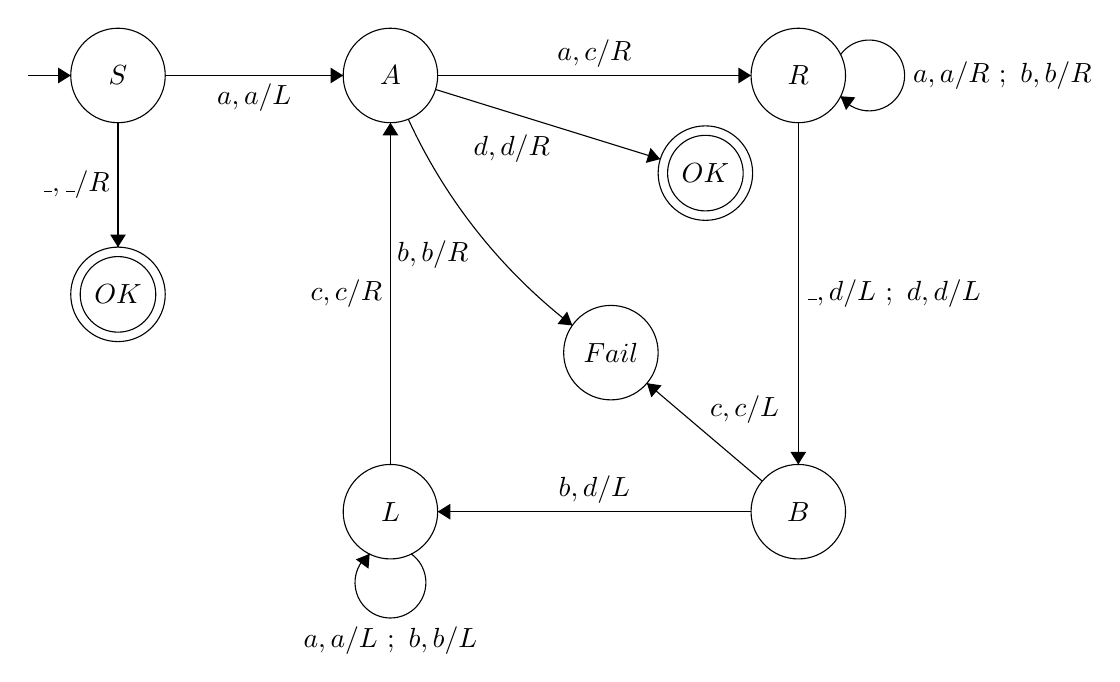
\begin{tikzpicture}[scale=0.2]
    \tikzstyle{every node}+=[inner sep=0pt]
    \draw [black] (47.6,-11.9) circle (3);
    \draw (47.6,-11.9) node {$OK$};
    \draw [black] (47.6,-11.9) circle (2.4);
    \draw [black] (41.6,-23.3) circle (3);
    \draw (41.6,-23.3) node {$Fail$};
    \draw [black] (27.6,-5.7) circle (3);
    \draw (27.6,-5.7) node {$A$};
    \draw [black] (53.5,-5.7) circle (3);
    \draw (53.5,-5.7) node {$R$};
    \draw [black] (53.5,-33.4) circle (3);
    \draw (53.5,-33.4) node {$B$};
    \draw [black] (27.6,-33.4) circle (3);
    \draw (27.6,-33.4) node {$L$};
    \draw [black] (10.3,-5.7) circle (3);
    \draw (10.3,-5.7) node {$S$};
    \draw [black] (10.3,-19.6) circle (3);
    \draw (10.3,-19.6) node {$OK$};
    \draw [black] (10.3,-19.6) circle (2.4);
    \draw [black] (30.6,-5.7) -- (50.5,-5.7);
    \fill [black] (50.5,-5.7) -- (49.7,-5.2) -- (49.7,-6.2);
    \draw (40.55,-5.2) node [above] {$a,c/R$};
    \draw [black] (53.5,-8.7) -- (53.5,-30.4);
    \fill [black] (53.5,-30.4) -- (54,-29.6) -- (53,-29.6);
    \draw (54,-19.55) node [right] {$\_,d/L\mbox{ };\mbox{ }d,d/L$};
    \draw [black] (50.5,-33.4) -- (30.6,-33.4);
    \fill [black] (30.6,-33.4) -- (31.4,-33.9) -- (31.4,-32.9);
    \draw (40.55,-32.9) node [above] {$b,d/L$};
    \draw [black] (27.6,-30.4) -- (27.6,-8.7);
    \fill [black] (27.6,-8.7) -- (27.1,-9.5) -- (28.1,-9.5);
    \draw (27.1,-19.55) node [left] {$c,c/R$};
    \draw [black] (28.923,-36.08) arc (54:-234:2.25);
    \draw (27.6,-40.65) node [below] {$a,a/L\mbox{ };\mbox{ }b,b/L$};
    \fill [black] (26.28,-36.08) -- (25.4,-36.43) -- (26.21,-37.02);
    \draw [black] (56.18,-4.377) arc (144:-144:2.25);
    \draw (60.75,-5.7) node [right] {$a,a/R\mbox{ };\mbox{ }b,b/R$};
    \fill [black] (56.18,-7.02) -- (56.53,-7.9) -- (57.12,-7.09);
    \draw [black] (30.47,-6.59) -- (44.73,-11.01);
    \fill [black] (44.73,-11.01) -- (44.12,-10.3) -- (43.82,-11.25);
    \draw (35.3,-9.42) node [below] {$d,d/R$};
    \draw [black] (39.15,-21.571) arc (-127.66889:-155.3298:34.996);
    \fill [black] (39.15,-21.57) -- (38.82,-20.69) -- (38.21,-21.48);
    \draw (32.58,-17.08) node [left] {$b,b/R$};
    \draw [black] (51.21,-31.46) -- (43.89,-25.24);
    \fill [black] (43.89,-25.24) -- (44.17,-26.14) -- (44.82,-25.38);
    \draw (50.09,-27.86) node [above] {$c,c/L$};
    \draw [black] (4.6,-5.7) -- (7.3,-5.7);
    \fill [black] (7.3,-5.7) -- (6.5,-5.2) -- (6.5,-6.2);
    \draw [black] (10.3,-8.7) -- (10.3,-16.6);
    \fill [black] (10.3,-16.6) -- (10.8,-15.8) -- (9.8,-15.8);
    \draw (9.8,-12.65) node [left] {$\_,\_/R$};
    \draw [black] (13.3,-5.7) -- (24.6,-5.7);
    \fill [black] (24.6,-5.7) -- (23.8,-5.2) -- (23.8,-6.2);
    \draw (18.95,-6.2) node [below] {$a,a/L$};
    \end{tikzpicture}
    \end{center}
    \newpage

    \item \begin{enumerate}
        \item Designate two new alternate languages that we will use to designate the first and second half of the string. Let {a,b} be the left language L and {c, d} be the right language R.

        \item Remember the character in the current cell, and write a terminal character '\#'.

        \item Move right one cell and remember the character in the cell while writing the character from the previous cell.

        \item Repeat steps (b)-(d) until the entire string has been shifted one space to the right and the TM head is sitting at the first empty cell after the input string. Write the terminal character \#.

        \item Return to the beginning of the string by moving left until you read the terminal character and then moving right once.

        \item aaaRead the character in the current cell and replace it with the corresponding symbol from L: a if the TM read a 0 and b if it read a 1.

        \item Move right until you reach a terminal character or a character in R. Then move left once.

        \item Replace the character in the current cell with the corresponding symbol from R: c if the TM read a 0 and d if it read a 1.

        \item Move left until you reach a symbol in L. Then move right once.

        \item If the current character isn't in R, repeat steps (f)-(j).

        \item Move left until you reach \#, then move right once. Remember the current character, replacing it with an \_.

        \item Move right until you reach a symbol in R.

        \item If the current symbol corresponds to the same symbol encoded in memory by language L,  replace the current cell with an \_, if they don't match, reject.

        \item Move left until you reach a \#.

        \item Move right until you reach a character in L. If you read \#, accept.

        \item Repeat steps (k)-(p).
    \end{enumerate}
    \newpage

    \item Let $P$ be the language $\{<N, R> | \; N$ is an NFA \& $R$ is a regular expression where $L(N) = L(R)\}$

    Then, let the following Turing Machine, $T$ decide $P$:

    $T = $ "On input $<N,R>$ where $N$ is an NFA and $R$ is a regular expression:
    \begin{enumerate}
        \item Use the algorithms from class to convert the regular expression $R$ to NFA $R_{NFA}$.

        \item Use subset construction to convert NFA $N$ to DFA $N_{DFA}$ and NFA $R_{NFA}$ to DFA $R_{DFA}$.

        \item Run the TM $EQ_{DFA}$ from lecture with inputs $N_{DFA}$ and $R_{DFA}$.

        \item If $EQ_{DFA}$ accepts, accept. If $EQ_{DFA}$ rejects, reject.
    \end{enumerate}

    \item We can show that $All_{DFA}$ is decidable by designing a decider for it. Let $D$ be this decider and define it as such:
    $D = $ "On input $M$ where $M$ is a DFA:
    \begin{enumerate}
        \item Using algorithm T from the emptiness problem in lecture, run algorithm T on $M$.
        \item if $L(M) = \emptyset$, reject. Otherwise, accept.
    \end{enumerate}

    \item Let us assume that $A_{101}$ is decidable, and $T_{101}$ is the turing machine that decides $A_{101}$. $T_{101}$ is the machine that simulates $A_{101}$ and accepts if $A_{101}$ accepts and rejects otherwise. Then, we will run the Diagonalize function, $D$ on $T_{101}$. $D<T_{101}>$ accepts if $<T_{101}>$ rejects and vice versa. But, since we can run $D<D<M>>$ on itself, we know that this will accept when it rejects and reject when it accepts, which is a contradiction, and therefore $A_{101}$ is undecideable.
\end{enumerate}
\end{document}
